\documentclass[../main.tex]{subfiles}

\usepackage[all,cmtip]{xy}
\usetikzlibrary{matrix}

\title{Capitolo 5 - Degenerations of Hodge structures}
\author{Edoardo Manini}
\date{Febbraio 20, 2025}

\begin{document}
\ifSubfilesClassLoaded{
\maketitle
\tableofcontents
}{}



Usually, families of varieties come with singular fibers and it is rather interesting to investigate what happens near such a fiber. Here we mostly consider 1-parameter degenerations, i.e. a family that is smooth over the punctured disk $\Delta^* = \Delta \setminus \{0\} $. The flat connection on any of the local systems coming from the cohomology of the smooth fibers over $\Delta^*$ acquires a logarithmic singularity
and its residue is related to the monodromy around the singular fiber.
A result by Schmid allows us to define a limiting Mixed Hodge structure on the cohomology of the nearby fiber which is related to the natural mixed Hodge structure on the central fiber of such degenerations.

\subsection{Residue maps}
We first define residue maps as we will use them frequently in the next sections.
The set up is as in the previous section, so let $Y= Y_1 \cup Y_2 \cup \cdots \cup Y_k$ be a simple normal crossing divisor inside a complex manifold X. Let $I = \{ i_1< \dots <i_m\}$, introduce
\begin{align*}
    Y_I &= Y_{i_1} \cap \cdots \cap Y_{i_{m}}; \\
    Y(I) &= \sum_{j \not\in I} Y_I \cap Y_j; \\
     a_I &\colon Y_I \hra X ;
\end{align*}
and define for $m \geq 0$, the \emph{codimension $m$ stratum} of $Y$ to be
\[
Y(0)=X, \qquad Y(m) = \coprod_{|I|=m}  Y_I, \qquad m=1,\dots,N 
\]
and let $a_m= \coprod_{|I|=m} a_I \colon Y(m) \ra X$ denote the natural map. Let us also define for later use $Y[m]$ the set of of points of $Y$ of multiplicity at least $m$.


We want to define residues along $Y_I$. Take a point $p \in Y_I \subseteq Y(m)$. All $m$ components $Y_i, i\in I$ pass through $p$, but maybe more if $p$ also belongs to the lower stratum $Y(m+1)$. We choose coordinates $(U,z_1,\dots ,z_n)$ centred at $p$ in which $Y$ has equation $z_1 \cdots z_k =0$ in such a way that $Y_{i_j} = \{ z_j = 0 \} $ for $j = 1,\dots ,m$, and such that the remaining $k - m$ components of $Y$ are given by the equations ${z_j = 0}$, $j = m + 1,\dots ,k$. Any local section $\omega$ of $\Omega^r_X(\log Y)$ can then be written as 
\[
\omega = \frac{dz_1}{z_1} \wedge \cdots \wedge\frac{dz_m}{z_m} \wedge \eta + \eta^\prime
\]
where $\eta$ has at most poles along components $Y_j , j \not\in I$, and $\eta^\prime$ is not divisible by the form $\frac{dz_1}{z_1}\wedge \cdots \wedge\frac{dz_m}{z_m} $. The restriction of $\eta$ to $Y_I$ is independent of the chosen adapted local coordinates. 

\begin{defn}
The residue map is
    \begin{align*}
    \res_I \colon \Omega^r_X( \log Y) &\to \Omega^{r-m}_{Y_I}( \log Y(I))  \\
          \omega &\mapsto \eta|_{Y_I} 
    \end{align*}
where $\omega = \frac{dz_1}{z_1} \wedge \cdots \wedge\frac{dz_m}{z_m}\wedge \eta + \eta^\prime$.
  \end{defn}

    
We note that
\[
d\omega = \frac{dz_1}{z_1} \wedge \cdots \wedge\frac{dz_m}{z_m}
\wedge (-1)^m d\eta + d\eta^\prime
\]
which implies that the residue map is compatible with the differentials, i.e. it is a morhpism of complexes. 

\begin{rem}
The residue map restricts to
\begin{align}
    \res_I \colon W_m\Omega^r_X( \log Y) &\to \Omega^r_{Y_I}[-m]
\label{res_I}
\end{align}
Indeed, if in the local description $\omega$ has weight $\leq m$, clearly $\eta|_{Y_I}$ is a holomorphic form.
\end{rem}

  \begin{lemma}\label{lemmaresiso}
      The residue map (\ref{res_I}) is surjective and induces an isomorphism of complexes of sheaves on $X$ supported on $Y$
      \begin{align}
          \res_m = \bigoplus_{|I|=m}\res_I \colon \Gr^W_m \Omega^\bullet_X(\log Y) \xrightarrow{\sim} (a_m)_* \Omega^\bullet_{Y(m)}[-m]. \label{resiso}
      \end{align}
  \end{lemma}
\begin{proof}
    We construct an inverse as follows. As before, fix an index set $I = {i_1,\dots ,i_m}, \quad 1 \leq i_1 < i_2 < \cdots < i_m \leq k$. Define
    \begin{align*}
        \rho_I \colon \Omega^r_X \to \Gr^W_m \Omega^{r+m}_X (\log Y) \\
        \rho_I (\beta) =\frac{dz_1}{z_1} \wedge \cdots \wedge\frac{dz_m}{z_m} \wedge \beta.
    \end{align*}
This map is well-defined, since, if $(V,w_1,\dots ,w_n)$ are other local coordinates in which $Y$ is given by $\{ w_1 \cdots  w_k = 0 \}$, the quotients $z_i/w_i$ are holomorphic and also the
forms $\frac{dz_i}{z_i}-\frac{dw_i}{w_i}$ are holomorphic, so that $\rho_I (\beta)$ in the $w$-coordinates differs from the expression in the $z$-coordinates by a form in $W_{m-1}\Omega^{r+m}_X (\log Y)$ and so is zero in the quotient. Also, the elements of the form $\beta = z_{i_j} \beta^\prime$, $\beta^\prime$ a local section of $\Omega^p_X$, and $dz_{i_j} \wedge \beta^{\prime\prime}$, $\beta^{\prime\prime}$ a local section of $\Omega^{p-1}_X$, map to zero so that the map $\rho_I$ induces a map of complexes $\Omega^\bullet_{Y_I}[-m] \to \Gr^W_m \Omega^\bullet_X(\log Y)$ which can be assembled for $|I| = m$ to give a morphism of complexes 
\[
(a_m)_*\Omega^\bullet_{Y(m)}[-m] \to \Gr^W_m \Omega^\bullet_X(\log Y).
\]
This is clearly an inverse for the residue map.
\end{proof}

We use this residue isomorphism to calculate the groups in the first page of the spectral sequence  associated to the weight filtration on $H^k(U, \C)$ which is 
\[
E^{-m,k+m}_1 = \HH^k(X, \Gr^W_m \Omega^\bullet_X(\log Y))
\]
By the above Lemma it is isomorphic to $H^{k-m}(Y(m), \C)$. 

We can picture the $E_1^{\bullet,\bullet}$-page as 
\begin{center}
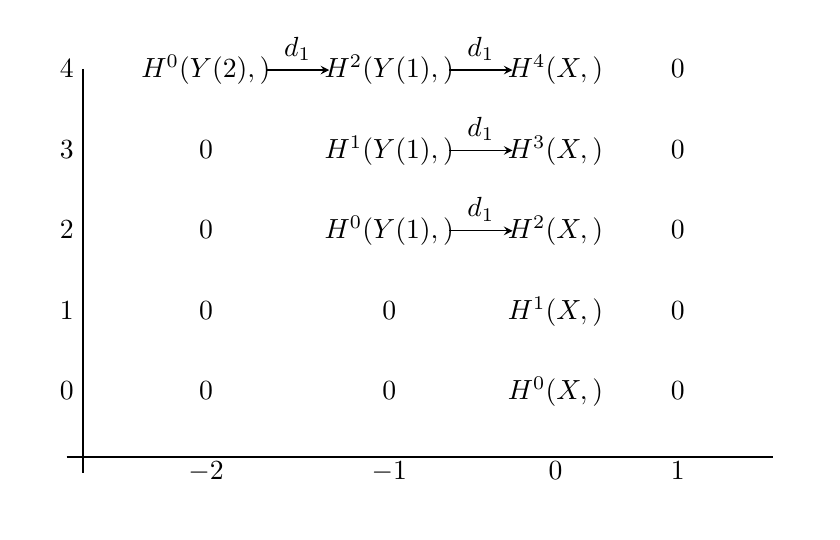
\begin{tikzpicture}
  \matrix (m) [matrix of math nodes,
    nodes in empty cells,nodes={minimum width=5ex,
    minimum height=5ex,outer sep=-5pt},
    column sep=3ex,row sep=1ex]{
    4   & H^0(Y(2),\CC) & H^2(Y(1),\CC) & H^4(X,\CC) & 0 & \\
    3   &      0        & H^1(Y(1),\CC) & H^3(X,\CC) & 0 & \\
    2   &      0        & H^0(Y(1),\CC) & H^2(X,\CC) & 0 & \\
    1   &      0        &        0      & H^1(X,\CC) & 0 & \\
    0   &      0        &        0      & H^0(X,\CC) & 0 & \\
    \quad\strut &   -2            &  -1  &  0  & 1    & \strut \\};
  \draw[-stealth] (m-3-3.east) -- node[anchor=south] {$d_1$} (m-3-4.west) ;  
   \draw[-stealth] (m-2-3.east) -- node[anchor=south] {$d_1$} (m-2-4.west) ;  
    \draw[-stealth] (m-1-3.east) -- node[anchor=south] {$d_1$} (m-1-4.west) ;  
  \draw[-stealth] (m-1-2.east) -- node[anchor=south] {$d_1$} (m-1-3.west) ;
\draw[thick] (m-1-1.east) -- (m-6-1.east) ;
\draw[thick] (m-6-1.north) -- (m-6-6.north) ;
\end{tikzpicture}
\end{center}


We want to recognize the differentials in the first page $d_1$ as certain known maps between the cohomology groups on the strata $Y(k)$. To this end, remember the inclusion maps $\delta_j^m\colon Y(m) \to Y(m-1)$ ($1 \leq j \leq m$)  defined in Section \ref{mhsncd}. Define now
\[
\gamma \defeq \bigoplus_{j=1}^m (-1)^{j-1} (\delta_j^m)_! \colon H^{k-m}(Y(m), \C)(-m) \to H^{k-m+2}(Y(m-1), \C)(-m+1)
\]
where we used the Gysin maps for $\delta_j^m$.
Recall that, for an inclusion of compact (real) manifolds $f \colon X^n \to Y^m$, the associated Gysin map is the composition $H^q(X) \xrightarrow{\sim} H_{n-q}(X) \xrightarrow{f_*} H_{n-q}(Y) \xrightarrow{\sim} H^{q+m-n}(Y)$ where the two isomorphisms are Poincarè isomorphisms.
If $f$ is an inclusion of compact K\"{a}hler manifolds $X^{2n}$, $Y^{2m}$, the Gysin map is $f_! \colon H^q(X) \to H^{q+2(m-n)}(Y)$. To endow it with the structure of a morphism of Hodge structures (i.e. of type $(0,0)$) we could perform a single Tate twist on either side 
\[
f_! \colon H^q(X)(n-m) \to H^{q+2(m-n)}(Y) \qquad f_! \colon H^q(X) \to H^{q+2(m-n)}(Y)(m-n)
\]
or one Tate twist on each side
\[
f_! \colon H^q(X)(-m) \to H^{q+2(m-n)}(Y)(-n)
\]
in order to get the same weight HS.
It is clear that the Tate twists in the definition of $\gamma$ are there to have Hodge structures of weight $k+m$ on either side.

We have the
\begin{proposition} \textup{\cite[Prop. 4.7]{PS08}}
    For all $m \geq 1$ the following diagram is commutative
     \begin{equation}\label{E1}
\xymatrix{
   E^{-m,k+m}_1(W) \ar[d]^-{d_1} \ar[r]^-{\res_m} & H^{k-m}(Y(m), \C)(-m) \ar[d]^-{-\gamma}    \\ 
   E^{-m+1,k+m}_1(W) \ar[r]^-{\res_m} & H^{k-m+2}(Y(m-1), \C)(-m+1)
}
\end{equation}
\end{proposition} 

Another immediate consequence of the residue isomorphism of Lemma \ref{lemmaresiso} is:

\begin{cor}
\begin{eqnarray*}    H^p(\Gr^W_m \Omega^\bullet_X(\log Y) )  =\left\{\begin{array}{ll} (a_m)_* \C_{Y(m)} &\quad p=m\\ 0&\quad\hbox{otherwise.}\end{array}\right.\\
\end{eqnarray*}
\end{cor}

from which we also deduce

\begin{cor}
 \[
 H^p(\Omega^\bullet_X(\log Y)) \cong (a_p)_* \C_{Y(p)} \qquad \forall p \in \Z. 
 \] 
 \end{cor}
  \begin{proof}
      We use the spectral sequence of the complex of sheaves $\Omega^\bullet_X( \log Y)$ with its filtration $W_\bullet$ as illustrated in the appendix \ref{sect_SpSeqfilt}. 
      This gives 
      \[
      E_1^{p,q} = H^{p+q}(\Gr^W_{-p} \Omega^\bullet_X(\log Y)) \Rightarrow H^{p+q}( \Omega^\bullet_X(\log Y))
      \]
Since $E_1^{p,q} = 0$ for $q \neq -2p$ then all differentials must be trivial and the sequence degenerates at $E_1$. Hence 
\[
  H^{k}( \Omega^\bullet_X(\log Y)) = \bigoplus_{p+q=k} E^{p,q}_\infty = E_1^{-k,2k} = H^{k}(\Gr^W_{k} \Omega^\bullet_X(\log Y)) =  (a_k)_* \C_{Y(k)} .
  \]
  \end{proof}


\subsection{Connections with Logarithmic Poles}

Let $X$ be a complex manifold and let $D = \sum_{i=1}^N D_i \subset X$ be a simple normal crossing divisor. Let $U = X \setminus D$.

\begin{defn} 
Let $\calE$ be a holomorphic vector bundle on $X$ and let $\nabla$ be a connection of $\calE|_U$, $\nabla \colon \calE|_U \to {\calE|}_{U} \otimes \Omega^1_X$ . Then $\nabla$ is said to \emph{have logarithmic poles along $D$} if it extends to a morphism
\[
\nabla \colon \calE \to  \calE  \otimes \Omega^1_X( \log D)
\]
which satisfies Leibniz’ rule $\nabla(fs) = s \otimes df + f\nabla s $, $\forall s$ sections of $\calE$ and $\forall f$ sections of $\calO_X$.
\end{defn} 
\begin{defn} 
For any irreducible component $D_k$ of $D$ the Poincaré residue map $R_k$ along $D_k$ is defined as follows. In
a coordinate chart with coordinates $z_1, \dots ,z_n$ such that $z_1 = 0$ is an equation for $D_k$, writing $\omega \in \Omega^1_X( \log D)$ locally as $\omega = \eta \wedge \frac{dz_1}{z_1} + \eta'$ with $\eta$, $\eta'$ not
containing $dz_1$, in this case the Poincaré residue map is
\begin{align*}
    R_k \colon \Omega^1_X(log D) &\to \calO_{D_k} \\
     \omega &\mapsto \eta |_{D_k}  
\end{align*}
    \end{defn} 
In particular $R_k(dz_1) = 0$ and $R_k(z_1 \omega) = 0$, where $\omega$ is a local section of $\Omega^1_X(\log D)$. So for local sections $f,m$ of $\calO_X(-D_k)$ and $\calE$ respectively one has $\nabla(fm) = m \otimes df + f\nabla m \in \ker(1_\calE \otimes R_k)$. This implies that the map $(1_\calE \otimes R_k) \circ \nabla$ induces a well-defined $\calO_{D_k}$-linear endomorphism since it is an $\calO_{X}$-linear morphism from $\calE \otimes \calO_{X}$ to $\calE \otimes \calO_{D_k}$ and it is trivial on $\calE \otimes \calO_{X}(-D_k)$. We denote it by
\[
\res_{D_k}(\nabla) \in \End(\calE \otimes \calO_{D_k}),
\]
and we call it the \emph{residue of the connection} along $D_k$.

Consider now the special case where $X$ is the unit disk $\Delta$ in the complex plane and $D$ is the origin. We let $\Delta^* = \Delta \setminus \{0\}$ and let T denote the monodromy automorphism of $ {\calE|}_{\Delta^*} $ determined by parallel transport along a counterclockwise loop around $0 \in \Delta$.
%
%We let $\mathfrak{H} := \{u \in \C | \Im(u) > 0 \}$
%be the upper half plane, which is the universal covering space of $\Delta^*$ via the map 
%\begin{align*}
%e \colon \mathfrak{H} &\to \Delta^* \\
%u &\mapsto e^{2\pi iu}
%\end{align*}
%
\begin{proposition}\label{T=res}
T can be extended to an automorphism of $\calE$ whose restriction $T_0$ to $\calE(0)$ is given by
\[
T_0 = e^{-2\pi i \res_0(\nabla)}.
\]
\end{proposition}
\begin{proof}
    Let $e_1, \dots, e_\mu$ be a local frame of $({\calE|}_{\Delta^*} )$. If $s=ey$ is a section, $\nabla(s)=e(dy+\omega y)$ where $\omega_{ij}=\Gamma_{ij}(b)db$ , where $\Gamma$ is the matrix of coefficients of the connection which is a function of $b$. Since the connection has only at most logarithmic poles, we have $\Gamma(b) = \frac{\Gamma_0}{b} + \Gamma_1(b)$ with $\Gamma_0 = \res_0(\nabla)$ a constant and $\Gamma_1$ a holomorphic function of $b$. Now a section $s=ey$ is flat if it is in $\ker \nabla$, i.e. if $y' = -\Gamma(b) y$ or $dy = -\Gamma(b)y db$.
    To calculate the monodromy we restrict to a circle $b=\rho e^{i \phi}$. Then $db = i \rho e^{i \phi} d\phi + e^{i \phi} d\rho$, and since on the circle $\rho=\rho_0$ is constant, $db = i \rho e^{i \phi} d\phi$. Substituting $b=\rho e^{i \phi}$ and $db = i \rho e^{i \phi} d\phi$ in $dy = -\Gamma(b)y db$ :
    \begin{align}
    dy &= -\left( \frac{\Gamma_0}{\rho e^{i\phi}}+ \Gamma_1 \right)  y i \rho e^{i \phi} d\phi  \nonumber \\
    dy &= -(i \Gamma_0 + i \rho e^{i \phi} \Gamma_1) y d\phi \label{equation} \tag{$\ast$}
    \end{align}
    
    The monodromy is calculated if we take a solution $Y$ of \eqref{equation} satisfying $Y|_{(\rho_0,\phi_0)} = Id$ to the point $(\rho_0,\phi_0 + 2 \pi)$.
    We see that \eqref{equation} depends continuously on $\rho$ and $\phi$, so there exists $\lim_{\rho \to 0} T = T_0$. 
    The solution of \eqref{equation} with $\rho =0$, i.e. $dy = -i \Gamma_0  y d\phi$ is $Y=e^{-i \Gamma_0 \phi}$ and 
    \[
    T_0 = Y|_{\phi=2\pi} = e^{-2\pi i \Gamma_0} = e^{-2\pi i \res_0(\nabla)}.
    \]
\end{proof}
On the other hand, for every bundle $(\calE, \nabla)$ on $\Delta^*$ equipped with a flat connection there exist extensions to a logarithmic connection over $\nabla$.
We have the
\begin{lemdef} \textup{\cite[Prop. 11.3]{PS08}}
There is a unique extension $(\tilde{\calE},\tilde{\nabla})$ of $(\calE,\nabla)$ to $\Delta$, such that $\tilde{\nabla}$ has logarithmic poles along $\{0\}$ and $\res_0(\nabla)$ has eigenvalues in the interval $[0,1)$.
This is called the \emph{canonical extension}.
\end{lemdef}


\subsection{Limiting Mixed Hodge Structure}

Recall that an endomorphism $T$ is called \emph{unipotent} if $(T-\id)^k=0$ for some $k$.
Now we specialize to the setting where the vector bundle $\calE$ arises from a variation of Hodge structure over $\Delta \setminus \{0\}$.

So let $(\calE_\ZZ,\calF)$ be a polarized variation of Hodge structure on $\Delta\setminus\{0\}$. 
Let $T\colon \calE_\ZZ \to \calE_\ZZ$ denote the monodromy automorphism defined by parallel transport along a counterclockwise loop about $0 \in \Delta$. Then $T$ induces an automorphism of $\calE := \calE_{\CC} \otimes \calO_{\Delta*}$. Let $T$ be in the Jordan normal form, i.e. choose a basis in which this automorphism consists of Jordan blocks
\[    
\begin{pmatrix}
\lambda & 1 &  &  \\ 
  & \ddots & \ddots & \\
   &  &  \lambda & 1\\
& & & \lambda
\end{pmatrix}.
\]
The following theorem gives an important property of $T$.

\begin{theorem}[Monodromy theorem] \label{monodromythm} \textup{\cite[Lemma 4.5, Thm. 6.1]{Sc73}} The monodromy operator $T$ is quasi-unipotent, i.e. the eigenvalues of $T$ are all roots of unity. More precisely, $\exists l \in \NN$ s.t. $T^l$ is unipotent and the index of quasiunipotency, i.e. the maximum size of a Jordan block, is $m:=\max\{p-q\mid\calE^{p,q}\neq 0\}$, 
\[(T^l-\id)^{m+1}=0.\]
\end{theorem}

Now let  $\tilde{\calE}$ denote the canonical extension of $\calE$ to $\Delta$ and let $\calE_\infty=\tilde{\calE}|_{\{0\}}$ denote its central fibre. There is an integral structure $(\calE_\infty)_\ZZ$ on $\calE_\infty$, induced from $\calE_\ZZ$ by the canonical extension. 

Moreover, by \ref{T=res}, $T$ extends to an automorphism of $\tilde{\calE}$, whose restriction to $\calE_{\infty}$ is given by $\exp(-2\pi i \res_0(\nabla))$. Let $T_u=T^l$ be the unipotent part, and let
\[N := \log T_u =\sum_{i\ge 1} (-1)^{i+1}\frac1i(T_u-\id)^i\]
denote the logarithm of the unipotent part; this is well-defined since the right hand side is a finite sum as $(T_u - \id)$ is nilpotent.
Since N is nilpotent, by a linear algebra Lemma, we have a naturally defined weight filtration on the canonical fibre of $\calE$:
\begin{lemma} \textup{\cite[Lemma 6.4]{Sc73}} \label{WeightFilt}
     Given a nilpotent endomorphism $N$, s.t. $N^{n+1}=0$ of a finite dimensional vector space $V$, $dim(V)=\mu$, there exists a unique increasing filtration  $W$ called the \emph{weight filtration of $N$ centred at $n$} 
     \[
       W_0 \subseteq \cdots \subseteq W_{2n}
     \]
     of $V$ with the properties:
    \begin{enumerate}
       \item  $N(W_i) \subset W_{i-2} \qquad \forall i \geq 2$; 
       \item  the map $N^k \colon \Gr^W_{n+k} V \to \Gr^W_{n-k} V$
is an isomorphism for all $k \geq 0$.
    \end{enumerate}
\end{lemma}

\begin{proof}
    Let $u_1, \dots, u_\mu$ form a basis of $V$ s.t. the representative matrix of $N$ in this basis is made by Jordan blocks:
    \[    
N=\begin{pmatrix}
J_{0,q_1} &    &  \\ 
  & \ddots  & \\
& & J_{0,q_l}
\end{pmatrix},
J_{0,q_i}=\begin{pmatrix}
0 & 1 &        &        & \\ 
  & 0 & 1      &        & \\
  &   & \ddots & \ddots & \\
  &   &  & 0 & 1 \\
    &   &  &  & 0
\end{pmatrix}
\]
of size $q_i \leq n+1$. For a generic block of size $q$ we have $N(u_1)=0, N(u_2)=u_1, N(u_3)=u_2, \dots ,N(u_q)=u_{q-1} $.
To every vector of the base of a block $J_{0,q}$ we associate a weight $(i)$ in such a way that the weights are symmetric with respect to $n$ and $N(u_{(i)})=u_{(i-2)}$ for all $i =1, \dots, n-q+1$ and $N(u_{(n-q+1)})=0$ . In other words:
\begin{align*}
    \text{if $q=2r+1$ is odd} &: u_{(n-2r)}, \dots, u_{(n-2)},  u_{(n)},  u_{(n+2)}, \dots,  u_{(n+2r)} \\
    \text{if $q=2r$ is even} &: u_{(n-2r+1)}, \dots, u_{(n-1)}, u_{(n+1)}, \dots,  u_{(n+2r-1)} 
\end{align*}
Now define $W_k \defeq \langle \{ u_{(p)} | p \leq k \} \rangle \subseteq V$ the subspace generated by vectors of weight $\leq k$. The filtration  $0 \subseteq W_0 \subseteq \cdots \subseteq W_{2n}$ satisfies $N(W_i) \subset W_{i-2}$ $ \forall i \geq 2$ and
\[
\Gr_{n+k}^W = \frac{\langle \{ u_{(p)} | p \leq n+k \}\rangle}{\langle \{ u_{(p)} | p \leq n+k-1 \}\rangle} \cong \langle \{ u_{(p)} | p = n+k \}\rangle \xrightarrow{N^k}  \Gr_{n-k}^W \cong  \langle \{ u_{(p)} | p = n-k \}\rangle
\]
is an isomorphism because by symmetry of construction for every $u_{(n-k)}$ vector of the basis of weight $n-k$ there exists a unique $u_{(n+k)}$ s.t. $N^k(u_{(n+k)}) =u_{(n-k)} $.
\end{proof}

We can use this filtration to define a mixed Hodge structure on $\calE_{\infty}=\tilde{\calE}|_{\{0\}}$ as follows:


\begin{theorem}[Schmid's limiting mixed Hodge structure] \textup{\cite[Thm. 6.16]{Sc73}} \label{limmhsthm}
The subbundles given by the Hodge filtration
\[\shF^n\subseteq\shF^{n-1}\subseteq\cdots\subseteq\shF^1\subseteq\shF^0=\calH^n \defeq \calE\]
extend to holomorphic subbundles
\[\tilde{\shF}^n\subseteq\tilde{\shF}^{n-1}\subseteq\cdots\subseteq\tilde{\shF}^1\subseteq\tilde{\shF}^0= \tilde{\calH}^n \defeq \tilde{\calE}\]
over $\Delta$. Define a decreasing filtration  $F^{\bullet}_{\operatorname{lim}}$ of $\calE_\infty=\tilde{\calE}|_{\{0\}}$ by $F^k_{\operatorname{lim}}=\tilde{\shF}^k|_{\{0\}}$ and let $W_{\bullet}$ denote the weight filtration on $\calE_\infty$ induced by the restriction of $N$ to $\calE_\infty$. Then
\[(\calE_\infty,W_\bullet,F^\bullet_{\operatorname{lim}})\]
defines a mixed Hodge structure, called the \emph{limiting mixed Hodge structure}.
\end{theorem}



\subsection{The nearby and vanishing cycle functor}

We are going to see the construction of Schmid's limiting mixed Hodge structure in the case of 1-parameter semistable degenerations. In particular we are going to construct a CMHC whose associated MHS is the limiting one. 

Let $\Delta$ be the unit disc and let $b$ be a coordinate on $\Delta$. Assume that we have a projective (proper, holomorphic) map $f\colon X\ra \Delta$ onto $\Delta$ that is smooth away from a reduced simple normal crossing central fibre $Y=f^{-1}(0)$. Assume further that $X$ is smooth (a complex manifold), so that locally $f$ has the form $f=z_1\ldots  z_k$, for $z_i$ part of a set of local coordinates and that the irreducible components of $Y$ are compact K\"ahler.
We will call this set-up a \emph{Semistable Degeneration}.
Consider the following diagram:
\begin{equation} \label{diagramdeg}
\begin{tikzcd} 
 Y \arrow[dr, phantom, "\scalebox{1.5}{$\lrcorner$}" , very near start, color=black] \arrow[hookrightarrow]{r}{i} \arrow[d] & X \arrow[bend right=30,swap]{l}{r} \arrow[d,"f"]  & \ar[l,hook', "j^y"]  U  \arrow[d]   & X_{\infty} \arrow[dl, phantom, "\scalebox{1.5}{$\llcorner$}" , very near start, color=black]  \arrow[l] \arrow[d, "f_{\infty}"] \arrow[bend right=30,swap]{ll}{k} \\
 \{0\}\arrow[hookrightarrow]{r} & \Delta  &  \Delta^*     \ar[l,hook'] &  \mathfrak{H} \arrow[l, "e"]
\end{tikzcd}
\end{equation}
Here $Y$ is the fibre over $0 \in \Delta$, $i$ the inclusion, $U = X \setminus Y$ , $\Delta^* = \Delta \setminus {0}$, $\mathfrak{H}$ the universal cover of $\Delta^*$, i.e. the upper half plane with the exponential map $e \colon \mathfrak{H} \to \Delta^*, \quad e(u)= e^{2 \pi i u} $ and $X_{\infty} = U \times_{\Delta^*} \mathfrak{H}$ the pullback. The map $j^Y$ is the inclusion and the map $k$ the projection $X_{\infty} \to U$ followed by $j^Y$.

The canonical fibre $X_{\infty}$ is homotopic to any fibre $X_b$ of $f$ since $f_{\infty}$ is differentiably a product. The total space $X$ is homotopy equivalent to $Y$ by a
fibre preserving retraction $r \colon X \to Y$. So the inclusion $i_b \colon X_b \to X$ followed by the retraction can be seen as the specialization map $r_b \colon X_b \to Y$.
The complex $(Rr_b)_* i_b^*\Z_X = \psi_f \Z_X$ is called the complex of nearby cocycles. 
We can describe its cohomology sheaves $\calH^q(\psi_f \ZZ_X)$. Since $\psi_f \ZZ_X$ is quasi-isomorphic to the constant sheaf at a general point of $Y$, we only need to find what the stalk is at a point where two or more irreducible components of $Y$ meet. The stalk $\calH^q(\psi_f \ZZ_X)_x$ is the limit over open neighbourhoods $U_x$ of $x$ of the integral cohomology groups of $r_b^{-1}(U_x)$:
\begin{equation} \label{cohomologysheaves}
\calH^q(\psi_f \ZZ_X)_x= \lim_{\to} H^q(r_b^{-1}(U_x))
\end{equation}

Note that, for a map of topological spaces $g \colon X \to Y$ and a complex of sheaves $\calF^\bullet \in D^+(X,\Z)$ we have $\HH^q(X, \calF^\bullet) =\HH^q(Y,Rg_*\calF^\bullet)  $.
Hence we obtain
\[
\HH^q(Y,\psi_f \Z_X) = \HH^q(Y,(Rr_b)_* i_b^*\Z_X ) = \HH^q(X_b, i_b^*\Z_X ) = H^q(X_b)
\]
and so $\psi_f \Z_X$ gives a rather elaborate way to calculate the cohomology of the smooth fibre.

\begin{lemma}\textup{\cite[Lemma 11.12]{PS08}} \label{quasiisonearby}
    The complex of nearby cocycles is quasi-isomorphic to
$i^*Rk_*(k^* \Z_X)$.
\end{lemma} 
Motivated by this Lemma, we define:
\begin{defn} \label{defNearbyVanishing}
    The functor $\psi_f \colon D^+(X,\Z) \to D^+(Y, \Z)$ from the derived category of sheaves of abelian groups on $X$ to the derived category of sheaves of abelian groups on $Y$
is defined by, for $\calF^\bullet \in D^+(X, \Z)$,
\[
\psi_f (\calF^\bullet) = i^* Rk_*(k^*(\calF^\bullet)).
\]
This is the \emph{sheaf of nearby cycles} of $\calF^\bullet$. 
One has a natural (unit of adjunction) morphism of complexes
\[
\calF^\bullet \to Rk_*k^*\calF^\bullet
\]
and hence a natural morphism of complexes
\[
sp \colon i^*\calF^\bullet \to \psi_f (\calF^\bullet).
\]
The cone of this map in $D^+(Y, \Z)$ is 
\[
\phi_f (\calF^\bullet) = cone^\bullet(sp) = i^*\calF^{\bullet+1} \oplus \psi_f \calF^\bullet,
\]
the \emph{sheaf of vanishing cycles} of  $\calF^\bullet$.
\end{defn} 
Inclusion on the second factor induces the canonical map $can \colon \psi_f (\calF^\bullet) \to \phi_f (\calF^\bullet)$
which occurs in the triangle for the cone
\[
\xymatrix{
i^*\calF^\bullet \ar[rr]^{sp} && \psi_f (\calF^\bullet)  \ar[dl]^{can}  \\
&\phi_f (\calF^\bullet) \ar[ul]^{[1]}  &
}
\]
where the left hand side map is the projection on the first factor and has as target the complex shifted by $1$.

%Note that in diagram \ref{diagramdeg} one may as well restrict $f$ to a small disk around $0$ and replace the map $e \colon \mathfrak{H} \to \Delta^*$ by its restriction to a subset $\{u \in \mathfrak{H} | Im(u) > K \}$ for some $K \in \RR$, $K > 0$. The map $h \colon X_\infty \to X_\infty$ given by $h(x,u) = (x, u + 1)$ satisfies $k \circ h = k$, hence we have an automorphism $h^*$ of $Rk_*k^*\calF^\bullet$ and of $\psi_f\calF^\bullet$. The formula for the monodromy becomes
%\[
%T := (h^*)^{-1} \colon \psi_f \calF^\bullet \to \psi_f \calF^\bullet
%\]
%The inverse is put here because $T$ follows a counterclockwise loop. We have an induced monodromy action on $\phi_f\calF^\bullet$, also denoted by $T$. Note that $(T -I)\circ sp = 0$, and we call \emph{variation map} the map
%\[
%var : \phi_f \calF^\bullet \to \psi_f \calF^\bullet
%\]
%defined by $var(x,y) = Ty - y$ for local sections $x,y$ of $i^*\calF^\bullet[1]$ and $\psi_f \calF^\bullet$ respectively. It is a morphism of complexes such that 
%\[
%T -I = var \circ  can \quad \text{on } \psi_f \calF^\bullet.
%\]
%Then also $can \circ var = T - I$ on $\phi_f \calF^\bullet$.
Under the assumption that all components of $Y$ are K\"ahler we are going to construct (cohomological) mixed Hodge complexes of sheaves $\psi_f^{\calH dg}$ and $\phi_f^{\calH dg}$ on $Y$ such that in the derived category of bounded above complexes of sheaves of $\QQ$-vector spaces on $Y$ we have $[\psi^{\calH dg}_f]_\QQ \simeq \psi_f \QQ_X$ and $[\phi^{\calH dg}_f]_\QQ \simeq \phi_f \QQ_X$; moreover we’ll show that there is an exact sequence of mixed Hodge complexes of sheaves
\[
0 \lra \calH dg^\bullet(Y) \lra [\psi^{\calH dg}_f]_\QQ \xrightarrow{can} [\phi^{\calH dg}_f]_\QQ \lra 0 .
\]
By Lemma \ref{quasiisonearby} this will put a mixed Hodge structure on the cohomology of $X_\infty$ which by definition is the limit mixed Hodge structure.



\subsection{Cohomological Mixed Hodge Complex of the Limiting Mixed Hodge Structure} \label{Sect.CMHC.LMHS}

We are going to construct (the $\C$-part of) a cohomological mixed Hodge complex CMHC $A^\bullet$ which will give us a MHC whose MHS is the limiting mixed Hodge structure on the cohomology of the nearby fiber, as defined by Thm. \ref{limmhsthm} . Moreover, we will see that there is a close relationship between $A^{\bullet}$ and $B^{\bullet}$, (the $\C$-part of) the cohomological mixed Hodge complex  we introduced in Sect. \ref{mhsncd} to put a MHS on the cohomology of a NCD singular variety. 

We know that the hypercohomology of the complex of sheaves of nearby cocycles gives us the cohomology of the nearby fibre :
\[
\HH^q(Y,\psi_f \C_X) = H^q(X_b, \C).
\]

\subsubsection{Relative De Rham complex}

We first construct a complex of sheaves on $Y$ which is quasi-isomorphic to $\psi_f \C_X$ but which is closer in nature to the complexes occurring in mixed Hodge theory, namely the relative de Rham complex on $X$ with logarithmic
poles along $Y$:
\[
R^\bullet := \Omega^\bullet_{X/\Delta}(\log Y) \defeq \frac{\Omega^\bullet_X(\log Y)}{f^*\Omega^1_\Delta(\log 0) \wedge \Omega^{\bullet-1}_X (\log Y)} \in D^+(X,\Z).
\]
By \cite[Thm 11.16]{PS08}  we have that $\psi_f \C_X$ is isomorphic in the derived category to $R^\bullet|_Y := \Omega^\bullet_{X/\Delta}(\log Y) \otimes \calO_Y$ so that $\HH^k(Y,\psi_f \C_X) \cong \HH^k(Y,R^\bullet|_Y) $.
Hence we reduced our problem to make  $R^\bullet|_Y$ a CMHC, i.e. we want to find two filtrations $W_\bullet, F^\bullet$ s.t. for every $m$, $\Gr_m^W R^\bullet|_Y$ is a Hodge complex of sheaves of weight $m$.
We first may try and define
\[
W_k R^\bullet|_Y \defeq im(W_k \Omega^\bullet_X(\log Y) \hra R^\bullet|_Y) = \frac{W_k \Omega^\bullet_X(\log Y)}{f^*\Omega^1_\Delta(\log 0) \wedge \Omega^{\bullet-1}_X (\log Y)} \otimes \calO_Y
\]
where the increasing filtration $W$ on $L^\bullet \defeq \Omega^\bullet_X(\log Y) $ is by order of poles:

\begin{eqnarray*}
W_k\Omega^{p}_{{X}}(\log Y) =  \left\{\begin{array}{ll} 
 0 &\quad k < 0 \\ 
\Omega^{k}_{{X}}(\log Y)\wedge \Omega^{p-k}_{{X}} &\quad 0 \leq k \leq p \\  
\Omega^{p}_{{X}}(\log Y) &\quad k>p  \end{array}\right.\\
\end{eqnarray*}

To see if $\Gr_m^W R^\bullet|_Y$ is a Hodge complex of sheaves of weight $m$, we need to see if we have a pure HS of wt. $k+m$ on  $\HH^k(\Gr_m^W R^\bullet|_Y)$.
Let us then calculate the cohomology sheaves of  $\Gr_m^W R^\bullet|_Y$. By definition of $R^\bullet|_Y$ we have an exact sequence 
\[
\Omega^{\bullet-1}_{{X}}(\log Y)|_{Y} \xrightarrow{\theta}  \Omega^{\bullet}_{{X}}(\log Y)|_{Y} \twoheadrightarrow  R^\bullet|_Y \ra 0
\]
where $\theta(\omega)=\frac{db}{b} \wedge \omega$. We see that $\theta$ descends to a map $\theta \colon W_k L^p|_Y \to W_{k+1} L^{p+1}|_Y $, so it induces well-defined maps $\theta \colon \Gr^W_k L^{p+k}|_Y \to \Gr^W_{k+1} L^{p+k+1}|_Y $. Hence we have a sequence of sheaves, a priori not exact
\begin{align}
0 \ra \Gr^W_0 L^{p}|_Y \xrightarrow{\theta}  \Gr^W_1 L^{p+1}|_Y \xrightarrow{\theta}  \Gr^W_2 L^{p+2}|_Y \xrightarrow{\theta} \cdots \label{GrSeq}
\end{align}
Applying residue isomorphisms \eqref{resiso} from lemma \ref{lemmaresiso}, we obtain 
\begin{align}
0 \ra \Omega^p_{X|_Y} \ra (a_1)_* \Omega^p_{Y(1)} \ra (a_2)_* \Omega^p_{Y(2)} \ra \cdots  \label{AltSumSeq}
\end{align}
which is an exact sequence since the maps are alternating sums of restriction maps.
This can be seen since the maps in \eqref{AltSumSeq} are the composition of $\rho = \res^{-1}$, the inverse of the residue described in the proof of Lemma \ref{lemmaresiso}, followed by $\theta$, and then again $\res$. For example for $k=1$, letting
\[
\eta = (\eta_1, \eta_2, \dots, \eta_k ) \in (a_1)_*\Omega^p_{Y(1)} = \bigoplus_{j=i, \dots, k} (i_j)_*\Omega^p_{Y_j},
\]
we have $\rho(\eta) = \frac{dz_1}{z_1} \wedge \eta_1 + \dots + \frac{dz_k}{z_k} \wedge \eta_k$ and
\begin{align*}
 \theta(\rho(\eta)) = \frac{db}{b} \wedge \rho(\eta) = \left( \sum_{j=1}^k \frac{dz_j}{z_j} \right) \wedge \left( \sum_{j=i}^k \frac{dz_j}{z_j} \wedge \eta_j \right) =  \sum_{j=i}^k \left(  \sum_{i \neq j} \frac{dz_i}{z_i} \wedge \frac{dz_j}{z_j} \wedge \eta_j   \right)
\end{align*}
Hence
\begin{align*}
    \res( \theta(\rho(\eta))) = \res \left( \sum_{i < j} \left( \frac{dz_i}{z_i} \wedge \frac{dz_j}{z_j} \wedge (\eta_j - \eta_i) \ \right)   \right) = ( \eta_j|_{ij} - \eta_i|_{ij} )_{i<j} \in  (a_2)_* \Omega^p_{Y(2)}
\end{align*}
and this is equal to $({\delta_1^2}^* - {\delta_2^2}^*)(\eta)$. Analogously for every $k$ one sees that the maps in \eqref{AltSumSeq} are just alternating sum of restriction maps.


Hence also (\ref{GrSeq}) is exact. Now again by definition we have the exact sequence
\begin{align*}
\Gr^W_{m-1} L^{\bullet-1}|_Y \xrightarrow{\theta}  \Gr^W_m L^{\bullet}|_Y \twoheadrightarrow  \Gr^W_m R^{\bullet}|_Y \xrightarrow{} 0 
\end{align*}
which fits in the following splitting of the long exact sequence \eqref{GrSeq}:
\begin{equation*}
\begin{tikzcd} 
   \Gr^W_{m-1} L^{\bullet-1}|_Y  \arrow[r, "\theta"]  & \Gr^W_{m} L^{\bullet}|_Y \arrow[rr, "\theta"] \arrow[dr,two heads]  & &  \Gr^W_{m+1} L^{\bullet+1}|_Y \arrow[r, "\theta"]  & \Gr^W_{m+2} L^{\bullet+2}|_Y \\
   &  & \Gr^W_m R^{\bullet}|_Y \ar[ur, "\theta"] \arrow[dr]  &  & \\
   & 0 \arrow[ur] & & 0 &
\end{tikzcd}   
\end{equation*}

By exactness of \eqref{GrSeq}, we deduce the exactness of the sequence 
\begin{align} \label{GrRLSeq}
0 \ra \Gr^W_m R^{\bullet}|_Y \xrightarrow{\theta}  \Gr^W_{m+1} L^{\bullet+1}|_Y \xrightarrow{\theta}  \Gr^W_{m+2} L^{\bullet+2}|_Y.
\end{align}  
We obtain 
\begin{lemma} \label{Lemmaexactsequence}
    The following sequence of complexes of sheaves is exact
\begin{align}
0 \ra \Gr^W_m R^{\bullet}|_Y \ra (a_{m+1})_* \Omega^{\bullet-m}_{Y(m+1)} \xrightarrow{\delta} (a_{m+2})_* \Omega^{\bullet-m}_{Y(m+2)}. \label{GrOmegaSeq}
\end{align}
\end{lemma}
\begin{proof}
    We just apply residue isomorphisms to the sequence \eqref{GrRLSeq}.
\end{proof} 
The sequence is nothing but
\begin{equation*}
\begin{tikzcd}
 & 0 \arrow[d] & 0 \arrow[d] & 0  \arrow[d]  \\
0 \arrow[r] & \Gr^W_m R^{m}|_Y \arrow[r]   \arrow[d,"d"] & (a_{m+1})_* \Omega^{0}_{Y(m+1)} \arrow[r,"\delta"]  \arrow[d,"d"] & (a_{m+2})_* \Omega^{0}_{Y(m+2)}  \arrow[d,"d"] \\
0 \arrow[r] & \Gr^W_m R^{m+1}|_Y \arrow[r]  \arrow[d,"d"]   & (a_{m+1})_* \Omega^{1}_{Y(m+1)} \arrow[r,"\delta"] \arrow[d,"d"] & (a_{m+2})_* \Omega^{1}_{Y(m+2)} \arrow[d,"d"] \\
 & \vdots & \vdots & \vdots
\end{tikzcd}
\end{equation*}
from which we see that $H^m(\Gr^W_m R|_Y^\bullet) \cong \ker((a_{m+1})_* \C_{Y(m+1)} \ra (a_{m+2})_* \C_{Y(m+2)}) \cong \C_{Y[m+1]} $ and $H^{m+q}(\Gr^W_m R|_Y^\bullet)= H^q(\Omega^\bullet_{Y[m+1]})=0$ if $q \neq 0$.
In particular, since $Y[1]=Y$, the inclusion $0 \to \CC_Y \hra \Gr^W_0 R|_Y^0 \to \Gr^W_0 R|_Y^1 \to \cdots$ induces a quasi-isomorphism between $\C_Y$ and $\Gr^W_0 R|_Y^\bullet$. In other words, $\Gr^W_0 R|_Y^\bullet$ is a resolution of $\C_Y$. In general we do not have a pure HS of weight $k$ on $\HH^k(\Gr^W_0 R|_Y^\bullet) = \HH^k(Y,\C_Y) = H^k(Y,\C)$ since $Y$ is in general non-smooth.
Nevertheless, this helps us get a resolution of $R|_Y^\bullet = 
\Omega^\bullet_{X/\Delta}(\log Y) \otimes \calO_Y$ as follows.

\subsubsection{The monodromy weight spectral sequence}

Consider the double complex with three filtrations $(A^{\bullet, \bullet}, d_>, d_\wedge, W(M), W, F)$ where
\[
A^{p,q}= \frac{\Omega^{p+q+1}_{{X}}(\log Y)}{W_q \Omega^{p+q+1}_{{X}}(\log Y)} = \frac{L^{p+q+1}}{\Omega_X^{p+1} \wedge L^q}  
\]
and the first differential is the usual holomorphic de Rham differential while the second differential is given by $\theta$, i.e. wedging with $\dlog f = f^*\dlog b$.
The two increasing filtrations $W$, $W(M)$ to which we refer to as the \emph{weight filtration}, respectively the \emph{monodromy
weight filtration} and the decreasing (\emph{Hodge}) filtration $F$ are given by the rules:
\begin{align*}
W_r A^{p,q} = \frac{W_{r+q+1} \Omega^{p+q+1}_{{X}}(\log Y) }{W_q\Omega^{p+q+1}_{{X}}(\log Y)} &= 
 \left\{\begin{array}{ll} 
 0 &\quad r \leq -1 \\ 
 \frac{ \Omega_X^{p-r} \wedge  L^{r+q+1} }{ \Omega_X^{p+1} \wedge  L^{q} } &\quad 0 \leq r \leq p - 1 \\
 A^{p,q} &\quad r \geq p \end{array}\right.\\
W(M)_rA^{p,q} = \frac{W_{r+2q+1} \Omega^{p+q+1}_{{X}}(\log Y)}{W_q\Omega^{p+q+1}_{{X}}(\log Y)} &= 
 \left\{\begin{array}{ll} 
 0 &\quad r \leq -q-1 \\ 
 \frac{ \Omega_X^{p-r-q} \wedge  L^{r+2q+1} }{ \Omega_X^{p+1} \wedge  L^{q} } &\quad -q \leq r \leq p-q-1 \\
 A^{p,q} &\quad r \geq p-q \end{array}\right.\\
F^rA^{p,q} &= 
 \left\{\begin{array}{ll} 
 A^{p,q} &\quad p \geq r \\ 
0 &\quad \text{otherwise}  \end{array}\right.\\
\end{align*}

Let $A^\bullet = \bigoplus_{p+q=\bullet}A^{p,q} $ denote the total complex. The three filtrations descend to this complex.
We define
\begin{align*}
\mu \colon R^p|_Y = \Omega^p_{{X}/\Delta}(\log Y)\otimes \calO_Y &\lra A^{p,0} \\
\omega &\mapsto (-1)^p \frac{db}{b} \wedge \omega = (-1)^p \theta(\omega) \mod W_0.
\end{align*}
This is injective because if $ (-1)^p \frac{db}{b} \wedge \omega=0 \in A^{p,0} = \frac{\Omega_X^{p+1}(\log Y)}{\Omega_X^{p+1}}$ then $\frac{db}{b} \wedge \omega \in \Omega_X^{p+1}$, i.e. $\frac{\omega}{b} \in \Omega_{X|_Y}^{p}$, i.e. $\omega =0$ in $\Omega_{X|_Y}^{p} \subset R|_Y^{p}$.
\begin{theorem}
$A^{\bullet}$ is quasi-isomorphic to $R^\bullet|_Y =\Omega^\bullet_{ X/\Delta}(\log Y)\otimes_{\shO_X} \calO_Y$.
\end{theorem} 
\begin{proof}
A morphism respecting two filtrations is called a bi-filtered quasi-isomorphism if the induced morphism between bi-graded pieces is a quasi-isomorphism.
We start by showing that  $\mu \colon (R^\bullet|_Y,W, F) \to (A^\bullet,W,F)$ is a bi-filtered quasi-isomorphism.
Indeed,
\[
A^\bullet = \bigoplus_{q \geq0} \left( \frac{L^{\bullet+1}}{W_q L^{\bullet+1}} \right), \qquad 
W_mA^\bullet = \bigoplus_{q \geq0} \left( \frac{W_{m+q+1}L^{\bullet+1}}{W_q L^{\bullet+1}} \right) \qquad \text{ and }
\]
\begin{equation} \label{formulaGrA}
\Gr^W_mA^\bullet = \bigoplus_{q \geq0} \left( \Gr^W_{m+q+1} L^{\bullet+1} \right) \underset{{\res}}{\cong}  \bigoplus_{q \geq0}(a_{m+q+1})_* \Omega^{\bullet-m-q}_{Y(m+q+1)} 
\end{equation}
and the morphism $\mu$, since it is compatible with the filtrations, descends to a morphism $\mu \colon \Gr_F^r \Gr^W_m R|_Y^\bullet \lra \Gr_F^r \Gr^W_m A^\bullet$ where 
\begin{align*}
\Gr_F^r \Gr^W_m R|_Y^\bullet =(0 \ra 0 \ra \cdots \ra 0 \ra &\underset{\text{r}}{\Gr^W_m R|_Y^r} \ra 0 \ra \cdots), \\
\Gr_F^r \Gr^W_m A^\bullet = (0 \ra 0 \ra \cdots \ra 0 \ra &\underset{\text{r}}{(a_{m+1})_* \Omega^{r-m}_{Y(m+1)}} \ra \underset{\text{r+1}}{(a_{m+2})_* \Omega^{r-m}_{Y(m+2)}} \ra \cdots)
\end{align*}
with cohomology sheaves
\begin{align*}
H^q(\Gr_F^r \Gr^W_m R|_Y^\bullet) &= 
\left\{\begin{array}{ll} 
 \Gr^W_m R|_Y^r &\quad q = r \\ 
0 &\quad \text{otherwise}  \end{array}\right.\\ \\
H^q(\Gr_F^r \Gr^W_m A^\bullet) &= 
\left\{\begin{array}{ll} 
 \ker \left( (a_{m+1})_* \Omega^{r-m}_{Y(m+1)} \ra (a_{m+2})_* \Omega^{r-m}_{Y(m+2)} \right)  &\quad q = r \\ 
0 &\quad \text{otherwise}  \end{array}\right.\\
\end{align*}
which, using the exact sequence \eqref{GrOmegaSeq} of Lemma \ref{Lemmaexactsequence}, we know to be isomorphic and the isomorphism is the one induced by the map $\theta$ (composed with the residue) in cohomology which coincides up to sign with $\mu$. 

Note that a bi-filtered quasi-isomorphism in general need not be a quasi-isomorphism, but for biregular filtrations (bounded above and below as in this case) this is always the case, therefore we are done.
\end{proof}
As a consequence of this theorem, we have
\[
\HH^n(Y,A^\bullet)= \HH^n(Y,R^\bullet|_Y).
\]
which we recall to be isomorphic to $\HH^n(Y,\psi_f \CC_X)$
We are going to see that $A^\bullet$ with the filtrations $W(M), F$ defined above is the $\CC$-part of a CMHC that computes the limiting mixed Hodge structure of Thm. \ref{limmhsthm} and therefore we have a MHS on its hypercohomology $\HH^n(Y,A^\bullet)= \HH^n(Y,\psi_f \C_X)= H^n(X_b, \C)$.
Indeed, since the vertical differential $d_\wedge=\theta$ sends $W(M)_rA^{p,q}$ to $W(M)_{r-1}A^{p,q+1}$, we have that
\[
\Gr^{W(M)}_r A^\bullet = \bigoplus_{q \geq 0 \atop r+2q+1 \geq q+1} \left( \Gr^W_{r+2q+1} L^{\bullet+1} \right) \underset{{\res}} {\cong}   \bigoplus_{q \geq0,-r}(a_{r+2q+1})_* \Omega^{\bullet-r-2q}_{Y(r+2q+1)}.
\]
To have a CMHC we need to show that $\Gr^{W(M)}_r A^\bullet$ is the $\C$-part of a pure Hodge complex of sheaves of weight $r$, i.e. that $F$  induces on  $\HH^k(\Gr^{W(M)}_r A^\bullet)$ a HS of weight $k+r$. Indeed, from the previous isomorphism we have
\[
\HH^k(\Gr^{W(M)}_r A^\bullet)  = \bigoplus_{q \geq0,-r}H^{k-r-2q}(Y(r+2q+1), \C).
\]
In order to get the right weight we perform a suitable Tate Twist (cfr. \ref{TateTwistDef}):
\[
\HH^k(\Gr^{W(M)}_r A^\bullet) (-r-q) = \bigoplus_{q \geq0,-r}H^{k-r-2q}(Y(r+2q+1), \C)(-r-q).
\]
In fact, since the irreducible components of $Y(r+2q+1)$ are smooth projective, i.e. compact K\"ahler, their cohomology has a HS and the weight is $k-r-2q -2(-r-q)=k+r$ as desired. 
One can also construct the rational part $A^\bullet_\QQ$ of the CMHC so that one has the 
\begin{theorem}  \textup{\cite[Thm. 11.22]{PS08}} \label{MHSonpsi}
    Let $f \colon X \to \Delta$ be a semistable degeneration.
    %proper holomorphic map from a complex manifold X to the unit disk in $\C$, smooth over the punctured disk. Suppose that $y = f^{-1}(0)$ is a reduced divisor with simple normal crossings on $X$ and that the irreducible components of $Y$ are K\"ahler. 
    The data
\[
\psi^{Hdg}_f := (\psi_f \Z_X,(A^\bullet_\QQ,W(M)),(A^\bullet,W(M),F))
\]
constitute a cohomological mixed Hodge complex of sheaves on $Y$.
This complex puts a mixed Hodge structure on the hypercohomology group $\HH^i(Y,\psi_f \Z_X) = H^i(X_\infty,\ZZ) = H^i(f^{-1}(b),\ZZ)$.
\end{theorem}
By Thm. \ref{MainThm} the (monodromy) weight spectral sequence (considered here after tensoring with $\C$) 
\begin{align} \label{monweightSpSeq}
 {}_{W(M)}{}{E_1^{-r,k+r}} = \bigoplus_{q \geq 0,-r } H^{k-r-2q}(Y(r+2q+1),\C)(-r-q) \Rightarrow H^k(X_b,\C). 
\end{align}
degenerates at $E_2$.


We deduce from \cite{PS08}, $\S$ 11.3.2, p. 280, that the morphisms $d_1$ are $\delta-\gamma$ where 
\begin{align*}
    \delta = \sum_{j=1}^{m} (-1)^{m+j-1}(\delta_j^{m})^* &\colon H^l(Y(m-1),\C) \to H^l(Y(m),\C) \\ 
    \gamma = \bigoplus_{j=1}^m (-1)^{j-1} (\delta_j^m)_!  &\colon H^l(Y(m),\C) \to H^{l+2}(Y(m-1),\C).
\end{align*}
This makes sense since, fixing $k$ and $r$, the map $d_1$ is
\begin{align*}
d_1 \colon   {E_1^{-r,k+r}} &\to {E_1^{-(r-1),(k+1)+(r-1)}} \\
d_1 \colon  \bigoplus_{q \geq 0,-r } H^{k-r-2q}(Y(r+2q+1),\C) &\to \bigoplus_{q \geq 0,-r+1 } H^{k-r-2q+2}(Y(r+2q),\C).
\end{align*}
If we choose the same $q$ on both sides the map raises the cohomology degree by two and lowers the codimension by one like the Gysin map $\gamma$. If we choose $q$ on the left side and $q+1$ on the right, the map fixes the cohomology degree and raises the codimension by one as $\delta$ does.


We can read off the Hodge numbers on the $E_2$-page
\[
h^{p,q}H^i(X_b,\C)=h^{p,q}\HH^i(A^\bullet)= \dim \Gr^p_F \Gr^{W(M)}_{p+q} \HH^i(A^\bullet)
\]
since $E^{-r,k+r}_2= \Gr_{k+r}^{W(M)} \HH^k(A^\bullet) $.

As a corollary of Thm. \ref{MHSonpsi}, by Thm. \ref{MainThm} we have that the Hodge spectral sequence 
\[
_F E_1^{pq} = \HH^{p+q}(X, \Gr_F^p R^\bullet|_Y)=H^q(Y,\Omega^p_{X/\Delta} (\log Y ) \otimes \calO_Y) \Rightarrow H^{p+q} (X_{\infty}, \CC)
\]
degenerates at $E_1$.

\begin{cor}
    Under the same hypotheses, for $b$ near $0$, the Hodge (Frolicher) spectral sequence 
    \[
    _F E_1^{pq} = H^q(X_b,\Omega^p_{X_b}) \Rightarrow H^{p+q} (X_b, \CC)
    \]
    degenerates at $E_1$.
\end{cor}
\begin{proof}
    Define $h^{p,q}(b) \defeq \dim H^q(X_b,\Omega^p_{X_b}) $ for $b \in \Delta$. By \cite{Voi07}[Cor. 9.19] for $b$ near $0$, $h^{p,q}(b) \leq h^{p,q}(0) $. For $b \neq 0$ one has $\Omega^p_{X/\Delta} (\log Y ) \otimes \calO_{X_b} \simeq \Omega^p_{X_b} $, so by the Hodge spectral sequence we have
    \[
    \sum_{p,q} h^{p,q}(b) \geq \sum_k \dim H^k(X_b,\C) \quad \text{ for } b \neq 0
    \]
    with equality if and only if the Hodge spectral sequence for $X_b$ degenerates at $E_1$. We have
    \[
    \sum_k \dim H^k(X_{\infty},\C) =  \sum_{p,q} h^{p,q}(0) \geq \sum_{p,q} h^{p,q}(b) \geq \sum_k \dim H^k(X_{b},\C)
    \]
    so equality must hold everywhere as $\dim H^k(X_{\infty},\C) = \dim H^k(X_{b},\C)$.
\end{proof}
As a consequence we see that 
\begin{align} \label{equalityHdgfiltr}
    \dim F^pH^k(X_{\infty}) =  \dim F^pH^k(X_{b}) \quad \text{ for } b \in \Delta^*.
\end{align}
For the Hodge-Grothendieck class we have
    \begin{align} \label{Hdg-Groth_class}
        \chi_{Hdg}(\psi_f^{Hdg}) &= \sum_{b \geq 1} (-1)^{b-1} \chi_{Hdg}(Y(b)) \cdot \left[ \sum_{a=0}^{b-1} \LL^a \right] \\
        &= \sum_{b \geq 1} (-1)^{b-1} \chi_{Hdg}( Y(b) \times \PP^{b-1})
    \end{align}
where $\LL = [\QQ(-1)] = H^2(\PP^1) \in K_0(\mathfrak{hs})$.
This can be seen by using the monodromy weight spectral sequence \eqref{monweightSpSeq}. 
We put $r+q=a, 2q+r+1=b, k-r-2q=c$. Then $a,c \geq 0, b \geq 1$, and since $q=b-a-1$, we have the restriction $0 \leq a \leq b-1$. We find:
    \begin{align*}
        \chi_{Hdg}(\psi_f^{Hdg}) &= \sum_{b \geq 1, c \geq 0} \sum_{a =0}^{b-1} (-1)^{c+b+1} [ H^c(Y(b))(-a)] \\
        &= \sum_{b \geq 1} (-1)^{b+1} \chi_{Hdg}(Y(b)) \cdot \left[ \sum_{a=0}^{b-1} \LL^a  \right].        
    \end{align*}
    From this, it follows that the Hodge-Euler polynomial is given by 
    \[
    e_{Hdg}(\psi_f^{Hdg})=\sum_{b \geq 1} (-1)^{b+1} e_{Hdg}(Y(b)) \frac{u^bv^b-1}{uv-1}.
    \]

\subsubsection{Steenbrink's long exact sequence}

There is an endomorphism of the double complex $A^{\bullet,\bullet}$, namely $\nu\colon A^{p,q} \ra A^{p-1,q+1}$,  given by the natural projection modulo $W_{q+1}$.

\begin{center}
\centerline{
\xymatrix{
\vdots & \vdots & \vdots &  \\
\frac{\Omega^3_{X}(\log Y)}{\Omega^1_X \wedge \Omega^2_{X}(\log Y)}\ar^d[r]\ar[u] & 
\frac{\Omega^4_{X}(\log Y)}{\Omega^2_X \wedge \Omega^2_{X}(\log Y)}\ar^d[r]\ar[u] &
\frac{\Omega^5_{X}(\log Y)}{\Omega^3_X \wedge \Omega^2_{X}(\log Y)}\ar[r]\ar[u] & \cdots
\\
\frac{\Omega^2_{X}(\log Y)}{\Omega^1_X \wedge \Omega^1_{X}(\log Y)}\ar^d[r]\ar^{\wedge \frac{db}b}[u] &
\frac{\Omega^3_{X}(\log Y)}{\Omega^2_X \wedge \Omega^1_{X}(\log Y)}\ar^d[r]\ar^{\wedge \frac{db}b}[u]\ar^{\nu}[lu] & 
\frac{\Omega^4_{X}(\log Y)}{\Omega^3_X \wedge \Omega^1_{X}(\log Y)}\ar[r]\ar^{\wedge \frac{db}b}[u]\ar^{\nu}[lu] & \cdots
\\
\frac{\Omega^1_{X}(\log Y)}{\Omega^1_{X}}\ar^d[r]\ar^{\wedge \frac{db}b}[u]& 
\frac{\Omega^2_{X}(\log Y)}{\Omega^2_{X}}\ar[r]\ar^{\wedge \frac{db}b}[u]\ar^{\nu}[lu] &
\frac{\Omega^3_{X}(\log Y)}{\Omega^3_{X}}\ar[r]\ar^{\wedge \frac{db}b}[u]\ar^{\nu}[lu] & \cdots 
\\
}
}
\end{center}
It commutes with $d_>$ and $d_\wedge$, therefore it induces an endomorphism of the associated simple complex $A^\bullet$ which we also denote by $\nu$. It maps $W(M)_r$ to $W(M)_{r-2}$ and $F^p$ to $F^{p-1}$. One can also define $\nu$ at the $\QQ$-level and at the $\ZZ$-level, so that it defines a morphism of mixed Hodge complexes of sheaves $\nu \colon \psi^{Hdg}_f \to \psi^{Hdg}_f(-1)$. The Tate twist is put here so that $\nu$ induces at the level of MHS a morphism (of type $(0,0)$) of mixed Hodge structures.

%One can use Thm. \ref{T=res} and the fact that $\nu$ coincides %with $-\res_0(\nabla)$, \cite[Thm. 11.21]{PS08}, to show that %$\nu$ is related to the monodromy operator $T$ by
%\[\log T=2\pi i \nu.\]
%%Hence the map
%\[
%\frac{\log T}{2 \pi i} = \nu \colon H^k(X_\infty) \to H^k(X_\infty)%(-1)
%\]
%is a morphism of mixed $\QQ$-Hodge structures.
We see that
\[\ker(\nu)^{p,q}= \frac{W_{q+1} \Omega^{p+q+1}_{{X}}(\log Y) }{W_q\Omega^{p+q+1}_{{X}}(\log Y)} = W_0 A^{p.q},\]
so $\ker(\nu)^{\bullet} = W_0 A^{\bullet}$ is itself a cohomological mixed Hodge complex with the filtrations $W(M)$ and $F$ induced from $A^{\bullet}$.
We also see that there is an isomorphism
\[\ker(\nu)^{\bullet}\cong B^\bullet,\]
where $B^\bullet$ is the cohomological mixed Hodge complex computing the mixed Hodge structure on the cohomology of $Y$ introduced in Sect. \ref{mhsncd}. This isomorphism is given by taking residues
\[\ker \nu^{p,q} = W_0A^{p,q}= \Gr^W_{q+1} \Omega^{p+q+1}_{{X}}(\log Y) \stackrel{\res}{\longrightarrow} (a_{q+1})_*\Omega^p_{{Y}^{(q+1)}} = B^{p,q} .\]
i.e. the injection
\[\operatorname{sp}\colon B^{\bullet}\lra A^\bullet\]
induces an injection on bigraded pieces and lifts to a map of CMHC 
\[
 sp^{Hdg} \colon \mathcal{H}dg^\bullet(Y) \lra \psi^{Hdg}_f.
\]
 Consequently we have that the specialization map
\[
sp \colon H^*(Y) \to H^*(X_\infty)
\]
is a morphism of mixed Hodge structures.

We denote the cokernel of the bifiltered injection of CMHC $\operatorname{sp} \colon B^\bullet \to A^\bullet$ by $\bar A^\bullet$.
We then have the
\begin{theorem} \cite[Thm. 4.5]{GKR17}\label{MHSonvanishing}
     \begin{enumerate}
         \item We have a short exact sequence of cohomological mixed Hodge complexes
         \[0\lra B^\bullet\stackrel{\operatorname{sp}}{\longrightarrow} A^\bullet \lra \bar A^\bullet \lra 0\]
         \item The inclusion $B^\bullet \to A^\bullet$ is isomorphic to $\C_Y \to \psi_f \C_X$ in $D^+(Y, \Z)$ and thus $\bar A^\bullet$ is isomorphic to $\phi_f \C_X$. This gives a mixed Hodge structure on the \emph{vanishing cohomology} $\HH^i(Y,\phi_f \C_X)$, and the sequence in (1.) turns the long exact sequence 
         \begin{align*}
             \cdots \to H^i(Y, \C) \to H^i(Y, \psi_f \C_X) \to H^i(Y, \phi_f \C_X) \to H^{i+1}(Y, \C) \to \cdots
         \end{align*}
into an exact sequence of mixed Hodge structures. 
     \end{enumerate} 
\end{theorem}
 We will call this long exact sequence \emph{Steenbrink's sequence}. 
 
\begin{proof} Exactness in (1) is clear. We have seen that the middle term is a cohomological mixed Hodge complex. For the kernel and cokernel it follows from the observation that after taking $\Gr^{W(M)}$ they can be written as a direct sum of shifted de Rham complexes on smooth varieties, we have
\begin{align*}
\Gr_r^{W(M)} \left(W_0 A^\bullet \right) &\simeq  \bigoplus_{{p+q=\bullet}\atop{2q+r+1=q+1}}  \Omega^{\bullet-r-2q}_{Y({2q+r+1})} = \left\{ \begin{array}{ll}
     \Omega^{\bullet+r}_{Y({-r+1})} &\quad r \leq 0 \\
     0 &\quad \text{otherwise} \\
\end{array} \right. , \\ \Gr_r^{W(M)} \bar A^\bullet &\simeq \bigoplus_{{p+q=\bullet}\atop{2q+r+1>q+1}}  \Omega^{\bullet-r-2q}_{Y({2q+r+1})} =  \bigoplus_{q \geq0,-r+1}(a_{r+2q+1})_* \Omega^{\bullet-r-2q}_{Y(r+2q+1)}
\end{align*}
The first part of (2) is clear, the remainder of (2) is standard given (1).
\end{proof}

\begin{cor}
The natural mixed Hodge structure on the \textbf{vanishing cohomology} $\HH^\bullet(Y,\phi_f^{Hdg})$ has Hodge-Grothendieck class
\begin{align*} 
    \chi_{Hdg}(\phi_f^{Hdg} ) &= \chi_{Hdg}(\psi_f^{Hdg})-\chi_{Hdg}(Y) \\
    &= \sum_{b \geq 1} (-1)^{b+1} \chi_{Hdg} (Y(b)) \cdot [\LL + \cdots + \LL^{b-1}]
\end{align*}
and its Hodge-Euler polynomial equals
\[
e_{Hdg}(\phi^{Hdg})= \sum_{b \geq 1} (-1)^{b+1} e_{Hdg} (Y(b)) \left( \frac{uv-u^bv^b}{1-uv} \right)
\]
\end{cor}
\begin{proof}
    By \ref{Hdg-characteristic-SES} the Hodge-Grothendieck characteristic class is the difference $\chi_{Hdg}(\psi_f^{Hdg})-\chi_{Hdg}(Y)$. Using \ref{HdgcharNCD} and \eqref{Hdg-Groth_class}, the result about the Hodge-Grothendieck class follows since 
    \begin{align*}
    \chi_{Hdg}(\phi_f^{Hdg} ) &= \chi_{Hdg}(\psi_f^{Hdg}) - \chi_{Hdg}(Y)  \\
    &= \sum_{b \geq 1} \left(  (-1)^{b+1} \chi_{Hdg}(Y(b)) \cdot \left[ \sum_{a=0}^{b-1} \LL^a \right] \right) - \sum_{b \geq 1} (-1)^b \chi_{Hdg} (Y(b))  \\
     &= \sum_{b \geq 1} (-1)^{b+1} \chi_{Hdg} (Y(b)) \cdot [\LL + \cdots + \LL^{b-1}]
    \end{align*}
and the result on the Hodge-Euler polynomial follows since 
\begin{align*}
    e_{Hdg} \left( \sum_{a=1}^{b-1} \LL^a \right) = \sum_{a=0}^{b-1} (e_{Hdg}(\LL))^a =  \sum_{a=0}^{b-1} (uv)^a = \frac{uv-u^bv^b}{1-uv}
 \end{align*}
\end{proof}

Considering the spectral sequence for $(\bar A^\bullet,W(M))$, as in \ref{thm:specseq}, with
\begin{equation}
\label{Wspecseq}
E^{-r,k+r}_1=\HH^{k}(X,\Gr^{W(M)}_{r}\bar A^\bullet) \Rightarrow \HH^{k}(X,\bar A^\bullet).
\end{equation}
From Theorem \ref{MainThm} we have that (\ref{Wspecseq}) is degenerate at $E_2$. As before the Poincar\'e residue map along $Y$ induces an isomorphism 
\[
\Gr^{W(M)}_{r} \bar A^\bullet 
= \bigoplus_{q>-1,-r}\Gr^{W}_{2q+r+1}\Omega^\bullet_X(\log Y)[1]
\stackrel{\sim}{\lra} \bigoplus_{q>-1,-r} \Omega^\bullet_{{Y}({2q+r+1})}[-2q-r].
\]
We thus have
\begin{align}
E^{-r,k+r}_1 =\bigoplus_{q>-1,-r} H^{k-2q-r}( Y({2q+r+1}),\CC)(-q-r).  \label{WspecseqTateTw}
\end{align}
The morphisms $d_1$ in the first page are $\delta-\gamma$, as for the weight spectral sequence $E_1$ for $A^\bullet$.

\begin{lemma} \textup{\cite[Lemma 4.7]{GKR17}} \label{lemWspecseq}
\begin{enumerate}
\item We have Poincar\'e duality for
\eqref{Wspecseq}, i.e., if we set $n=\dim X$, $k'=2n-k-2$, $r'=2-r$, we have an isomorphism
$$E_1^{-r,k+r}=(E_1^{-r',k'+r'}( n))^*$$
which is compatible with the respective differentials $d_1$ and $d_1^*$. 
In particular, it also holds when we replace $E_1$ by $E_\infty$. We obtain
$$h^{p,q}\HH^i(Y,\phi_f\CC_{\bar X}) = h^{n-p,n-q}\HH^{2n-2-i}(Y,\phi_f\CC_{\bar X}).$$
\item We have Poincar\'e duality also for the weight spectral sequence $E_1$ for $A^\bullet$ which yields
$$h^{p,q}\HH^i(Y,\psi_f\CC_{\bar X}) = h^{\dim Y-p,\dim Y-q}\HH^{2\dim Y-i}(Y,\psi_f\CC_{\bar X}).$$
\end{enumerate}
\end{lemma}

\begin{proof} 
For (1), we apply Poincar\'e duality to each summand in (\ref{WspecseqTateTw}). For $Z$ a compact complex manifold, Poincar\'e duality means 
\[
H^i(Z,\CC)=\Hom(H^{2\dim Z-i}(Z,\CC)( \dim Z),\CC).
\] 
Using $\dim Y(i)=n-i$, one remodels the resulting sum 
$$E_1^{-r,k+r}=\left( \bigoplus_{q>-1,-r} 
H^{2n-2-r-2q-k}( Y({2q+r+1}),\CC)( n-q-1) \right) ^*$$
by replacing $r,k,q$ by $r'=2-r$, $k'=2n-k-2$ and $q'=q+r-1$. In particular,
\[
\Gr_{p+q}^{W(M)} \HH^i(Y,\phi_f \C)= E_2^{i-p-q,p+q}=  (E_2^{-2-i+p+q,2n-p-q}(n))^*= (\Gr_{2n-p-q}^{W(M)} \HH^{2n-2-i}(Y,\phi_f \C)(n))^* ,
\]
so
\[
h^{p,q}\HH^i(Y,\phi_f\CC_{ X}) = h^{n-p,n-q}\HH^{2n-2-i}(Y,\phi_f\CC_{ X}).
\]
Part (2) is carried over in a similar way to (1).
\end{proof}

One can also prove the
\begin{theorem}\textup{\cite[Thm 11.40]{PS08}}
     The map $\nu$ induces isomorphisms
     \[
     \nu^r \colon \Gr^{W(M)}_{k+r} H^k(X_\infty, \QQ) \xrightarrow{\cong} \Gr^{W(M)}_{k-r} H^k(X_\infty, \QQ)(-r)
     \]
and the weight filtration $W(M)$ on $H^k(X_\infty, \QQ)$ coincides with the weight filtration of $N = \log T$ centred at $k$ from Lemma/Definition \ref{WeightFilt}.
\end{theorem}

Let us now show this machinery in an example.


\begin{es} 
\label{example-MHS5}
Consider the degenerating family given by 
\begin{align*}
    f \colon X=V(xyz-bz^3) \subset \PP^2 \times \Delta &\to \Delta \\
([x :y : z], b) &\mapsto b \\
\end{align*}
Note that the central fibre $Y$ of this family is exactly the variety $Y$ from Ex. \ref{example-MHS4}. See fig. \ref{fig:f2}.



\begin{figure}[!tbp]
  \begin{subfigure}[b]{0.4\textwidth}
    \includegraphics[width=\textwidth]{images/Nearby_Fibre_2.png}
    \caption{Nearby fibre}
    \label{fig:f1}
  \end{subfigure}
  \hfill
  \begin{subfigure}[b]{0.4\textwidth}
    \includegraphics[width=\textwidth]{images/Central_Fibre.png}
    \caption{Central fibre}
    \label{fig:f2}
  \end{subfigure}
  \caption{Semistable degeneration}
\end{figure}


The nearby fibre is a degree $3$ planar projective curve, hence an elliptic curve. The sheaf of nearby cocycles $\psi_f \ZZ_X$ is quasi-isomorphic to the constant sheaf at a general point of $Y$ and at a point where two $\PP^1$'s meet it has rank one in degree 0 and also rank one in degree 1 as we deduce from \eqref{cohomologysheaves}:
\[
\calH^q(\psi_f \ZZ_X)_x = \left\{\begin{array}{ll} 
 \ZZ &\quad q = 0,1 \\ 
0 &\quad \text{otherwise}  \end{array}\right.\\ \qquad \text{ for } x \in Y(2)
\]
The cohomology of the nearby fibre is the hypercohomology of the relative logarithmic de Rham complex $R|_Y^\bullet$:
\[0\lra\shO_Y\stackrel{d}{\longrightarrow} \left.\Omega^1_{X/\Delta}(\log Y)\right|_Y\lra 0\]
where $\Omega^2_{X/\Delta}(\log Y)|_Y=0$ because the relative dimension of $f\colon X\ra\Delta$ is one.

To obtain the weight filtration, we use the resolution of this complex by the double complex $A^{\bullet,\bullet}$ as given above. It takes the shape
\begin{center}
\centerline{
\xymatrix
{
0\\
\frac{\Omega^2_{X}(\log Y)}{\Omega^1_X \wedge \Omega^1_{X}(\log Y)}\ar^d[r]\ar^{\wedge \frac{db}b}[u] & 0\\
\frac{\Omega^1_{X}(\log Y)}{\Omega^1_{X}}\ar^d[r]\ar^{\wedge \frac{db}b}[u]& \frac{\Omega^2_{X}(\log Y)}{\Omega^2_{X}}\ar[r]\ar[u]&0\\
}}
\end{center}
The filtrations are

\begin{center}
\xymatrix
{
  & 0
  \\
0 \subset W_0 A^{\bullet,\bullet} = & \frac{\Omega^2_{X}(\log Y)}{\Omega^1_X \wedge \Omega^2_{X}(\log Y)} \ar^d[r] \ar^{\wedge \frac{db}b}[u] & 0 & & \subset W_1 A^{\bullet,\bullet} = A^{\bullet,\bullet} 
\\
& \frac{\Omega^1_{X}(\log Y)}{\Omega^1_{X}}\ar^d[r]\ar^{\wedge \frac{db}b}[u]& \frac{\Omega^1_X \wedge \Omega^1_{X}(\log Y)}{\Omega^2_{X}}\ar[r]\ar[u]&0
\\
}
\end{center}


\begin{center}
\xymatrix
{
& 0\\
0 \subset W(M)_{-1} A^{\bullet,\bullet} = & \frac{\Omega^2_{X}(\log Y)}{\Omega^1_X \wedge \Omega^2_{X}(\log Y)}\ar^d[r]\ar^{\wedge \frac{db}b}[u] & 0 & & \subset W(M)_0 A^{\bullet,\bullet} = W_0 A^{\bullet,\bullet} \subset A^{\bullet,\bullet} \\
& 0\ar^d[r]\ar^{\wedge \frac{db}b}[u]& 0\ar[r]\ar[u]&0\\
}
\end{center}


\begin{center}
\xymatrix
{
& 0\\
F^0 A^{\bullet,\bullet} = A^{\bullet,\bullet} \supset F^1 A^{\bullet,\bullet} = & 0\ar^d[r]\ar^{\wedge \frac{db}b}[u] & 0 & & \supset 0\\
& 0\ar^d[r]\ar^{\wedge \frac{db}b}[u]& \frac{\Omega^2_{X}(\log Y)}{\Omega^2_{X}} \ar[r]\ar[u]&0\\
}
\end{center}

Looking at graded pieces, using formula \eqref{formulaGrA}, we have that
\begin{align*}
    \Gr^{W(M)}_{-1} A^\bullet &\cong \bigoplus_{q \geq 1} (a_{2q})_* \Omega_{Y(2q)}^{\bullet+1-2q} = \left( 0 \ra (a_2)_*\calO_{Y(2)}  \ra 0 \right) \\
\Gr^{W(M)}_{0} A^\bullet &\cong \bigoplus_{q \geq 0} (a_{2q+1})_* \Omega_{Y(2q+1)}^{\bullet-2q} = \left( (a_1)_*\calO_{Y(1)} \ra (a_1)_*\Omega^1_{Y(1)}  \ra 0  \right) \\ 
\Gr^{W(M)}_{1} A^\bullet &\cong \bigoplus_{q \geq 0} (a_{2q+2})_* \Omega_{Y(2q+2)}^{\bullet-1-2q} = \left( 0 \ra (a_2)_*\calO_{Y(2)} \ra 0 \right). \\
\end{align*}
Through the residue isomorphisms, the $F$-filtration on $\Gr^{W(M)}_{r} A^\bullet$ gets sent to a filtration on $ \bigoplus_{q \geq0,-r}(a_{r+2q+1})_* \Omega^{\bullet-r-2q}_{Y(r+2q+1)}$ that only after performing the Tate twists $(-r-q)$ on each summand coincides with the usual Hodge filtration for the cohomology of a compact K\"{a}hler manifold.
For the calculation of the spectral sequence we can ignore the Tate twists, but we can not ignore them for the calculation of the Hodge numbers since they give shifts in the Hodge filtration.

We see that 
\begin{align*}
 \HH^k(\Gr^{W(M)}_{-1} A^\bullet) &= 
    \left\{\begin{array}{ll} 
 H^0(Y(2),\C) &\quad \quad k = 1 \\ 
0 &\quad \quad \text{otherwise}  \end{array}\right.\\ 
    \HH^k(\Gr^{W(M)}_0 A^\bullet) &= 
    \left\{\begin{array}{ll} 
 H^0(Y(1),\C) &\quad \quad k = 0 \\ 
  H^2(Y(1),\C) &\quad \quad k = 2 \\ 
0 &\quad \text{otherwise}  \end{array}\right.\\  \HH^k(\Gr^{W(M)}_1 A^\bullet) &= 
    \left\{\begin{array}{ll} 
 H^0(Y(2),\C)(-1) &\quad \quad k = 1 \\ 
0 &\quad \quad \text{otherwise}  \end{array}\right.\\
\end{align*}
Hence we construct the spectral sequence 
\[
 {}_{W(M)}{}{E_1^{-r,k+r}}= \HH^k(\Gr^{W(M)}_r A^\bullet)  = 
    \left\{\begin{array}{ll} 
 H^0(Y(1),\C) \cong \C^3 &\quad r = k = 0 \\ 
 H^2(Y(1),\C) \cong \C^3 &\quad r = 0, k = 2 \\
 H^0(Y(2),\C) \cong \C^3 &\quad r = -1, k = 1 \\
  H^0(Y(2),\C) \cong \C^3 &\quad r = k = 1 \\
0 &\quad \text{otherwise}  \end{array}\right.
\]
for which we can picture the $E_1^{\bullet,\bullet}$-page as 
\begin{center}
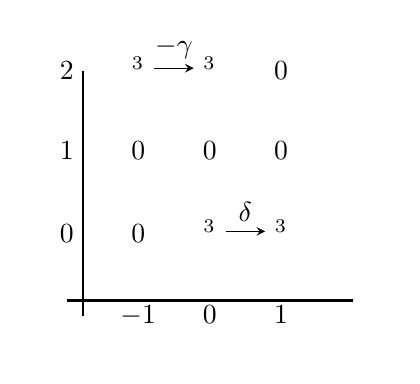
\begin{tikzpicture}
  \matrix (m) [matrix of math nodes,
    nodes in empty cells,nodes={minimum width=5ex,
    minimum height=5ex,outer sep=-5pt},
    column sep=1ex,row sep=1ex]{
          2     & \C^3 & \C^3 &  0   & \\
          1     &  0   &  0   &  0   & \\
          0     &  0   & \C^3 & \C^3 & \\
    \quad\strut &   -1  &  0  &  1  & \strut \\};
  \draw[-stealth] (m-3-3.east) -- node[anchor=south] {$\delta$} (m-3-4.west) ;  
  \draw[-stealth] (m-1-2.east) -- node[anchor=south] {$-\gamma$} (m-1-3.west) ;
\draw[thick] (m-1-1.east) -- (m-4-1.east) ;
\draw[thick] (m-4-1.north) -- (m-4-5.north) ;
\end{tikzpicture}
\end{center}
where the differential $E_1^{-1,2}=H^0(Y(2),\C) \to E_1^{0,2}=H^2(Y(1),\C)$ is the Gysin map $-\gamma$, i.e.
\begin{align*}
    H^0(Y(2))=\langle [1_{Y_{12}}], [1_{Y_{23}}],[1_{Y_{13}}]\rangle &\xrightarrow{-\gamma \defeq {\delta_2^2}_!-{\delta_1^2}_!} H^2(Y(1))=\langle [Y_{1}], [Y_{2}],[Y_{3}]\rangle \\
     [1_{Y_{12}}] &\mapsto [Y_{1}] - [Y_{2}] \\
     [1_{Y_{23}}] &\mapsto [Y_{2}] - [Y_{3}] \\
     [1_{Y_{13}}] &\mapsto [Y_{1}] - [Y_{3}] \\
\end{align*}
and the differential $E_1^{0,0}=H^0(Y(1),\C) \to E_1^{1,0}=H^0(Y(2),\C)$ is the restriction map $\delta$, i.e.
\begin{align*}
    H^0(Y(1))=\langle [1_{Y_{1}}], [1_{Y_{2}}],[1_{Y_{3}}] \rangle &\xrightarrow{\delta \defeq {\delta_1^2}^*-{\delta_2^2}^*} H^0(Y(2))=\langle [1_{Y_{12}}], [1_{Y_{23}}],[1_{Y_{13}}] \rangle \\
     [1_{Y_{1}}] &\mapsto - [1_{Y_{12}}] - [1_{Y_{13}}] \\
     [1_{Y_{2}}] &\mapsto [1_{Y_{12}}] - [1_{Y_{23}}] \\
     [1_{Y_{3}}] &\mapsto [1_{Y_{23}}] + [1_{Y_{13}}].  \\
\end{align*}
These two maps have both kernel of dimension one,
so the $E_2^{\bullet,\bullet}$-page looks like 
\begin{center}
\begin{tikzpicture}
  \matrix (m) [matrix of math nodes,
    nodes in empty cells,nodes={minimum width=5ex,
    minimum height=5ex,outer sep=-5pt},
    column sep=1ex,row sep=1ex]{
          2     & \C & \C &  0   & \\
          1     &  0   &  0   &  0   & \\
          0     &  0   & \C & \C & \\
    \quad\strut &   -1  &  0  &  1  & \strut \\};
\draw[thick] (m-1-1.east) -- (m-4-1.east) ;
\draw[thick] (m-4-1.north) -- (m-4-5.north) ;
\end{tikzpicture}
\end{center}
In other words 
\[
 {}_{W(M)}{}{E_2^{-r,k+r}}= \Gr^{W(M)}_{k+r} \HH^k(X,A^\bullet)=
    \left\{\begin{array}{ll} 
 \C &\quad r = k = 0 \\ 
 \C &\quad r = 0, k = 2 \\
  \C &\quad r = -1, k = 1 \\
  \C &\quad r = k = 1 \\
0 &\quad \text{otherwise}  \end{array}\right.
\]
Taking the sum along the anti-diagonals, we see that the cohomology groups are the ones of an elliptic curve, which is indeed the nearby fibre.
\[
\HH^i(A^\bullet)= \left\{\begin{array}{ll} 
 \C &\quad i = 0 \\ 
  \C^2 &\quad i = 1 \\
  \C &\quad i =2 \\
0 &\quad \text{otherwise} . \end{array}\right.
\]

We now come to the calculation of the Hodge numbers.


For $\HH^0(A^\bullet)$ we only have $\Gr^{W(M)}_0 \HH^0(A^\bullet) = \HH^0(A^\bullet) = \CC$ and the $F$-filtration is induced from the one on $H^0(Y(1),\CC)$ with no Tate twist ($-r-q=0$) hence only $\Gr_F^0$ survives.


For $\HH^1(A^\bullet)$ we have $\Gr^{W(M)}_0 \HH^1(A^\bullet) = \HH^1(A^\bullet) = \CC$ and $\Gr^{W(M)}_2 \HH^1(A^\bullet) = \HH^1(A^\bullet) = \CC$. The $F$-filtration on $\Gr_0^{W(M)}$ is induced from the one on $H^0(Y(2),\CC)$ with no Tate twist ($-r-q=0$) hence only $\Gr_F^0$ survives. The $F$-filtration on $\Gr_2^{W(M)}$ is induced from the one on $H^0(Y(2),\CC)$ with Tate twist $-r-q=-1-0=-1$ hence only $\Gr_F^{0+1}$ survives. 


For $\HH^2(A^\bullet)$ we only have $\Gr^{W(M)}_2 \HH^2(A^\bullet) = \HH^2(A^\bullet) = \CC$ and the $F$-filtration is induced from the one on $H^2(Y(1),\CC)$ with no Tate twist ($-r-q=0$) hence only $\Gr_F^1$ survives.

We also obtain the following Hodge numbers
\begin{eqnarray*}h^{p,q}\HH^2(A^\bullet)&=  \dim \Gr^p_F \Gr^{W(M)}_{p+q} \HH^2(A^\bullet)  &=\left\{\begin{array}{ll} 1 &\quad p=q=1\\ 0&\quad\hbox{otherwise,}\end{array}\right.\\
h^{p,q}\HH^1(A^\bullet)&= \dim \Gr^p_F \Gr^{W(M)}_{p+q} \HH^1(A^\bullet)   &=\left\{\begin{array}{ll} 1 &\quad p=q=0\hbox{ or }p=q=1\\ 0&\quad\hbox{otherwise,}\end{array}\right.\\
h^{p,q}\HH^0(A^\bullet)&= \dim \Gr^p_F \Gr^{W(M)}_{p+q} \HH^0(A^\bullet)  &=\left\{\begin{array}{ll} 1 &\quad p=q=0\\ 0&\quad\hbox{otherwise.}\end{array}\right.
\end{eqnarray*}

We note that the Hodge structure on $\HH^1(A^\bullet)$ is genuinely mixed, unlike the pure Hodge structure of an elliptic curve.
In this case the logarithm of the monodromy $N=\log T$ gives an isomorphism
     \[
     N \colon \Gr^{W(M)}_{2} \HH^1(A^\bullet) \xrightarrow{\cong} \Gr^{W(M)}_{0} \HH^1(A^\bullet)(-1)
\]
so that $N^2=0$ for $N \colon \HH^1(A^\bullet) \to \HH^1(A^\bullet) $. So $N$ is given by the matrix
$\begin{pmatrix} 0 & 1\\ 0 & 0\end{pmatrix}$ 
and $T=e^N=1+N\in \End(\HH^1(Y,\psi_f\CC))$ is given by the matrix
$\begin{pmatrix} 1 & 1\\ 0 & 1\end{pmatrix}$
which is the cohomological result of a Dehn twist.

We now want to give a description of Steenbrink's long exact sequence of mixed Hodge structures in this case, by combining the results of this example with those of Ex. \ref{example-MHS4}.

First we look at the mixed Hodge structure on the vanishing cohomology  $\HH^i(Y,\phi_f \C_X)$. We must calculate the spectral sequence:
\begin{equation}
\label{vanishingspecseq}
E^{-r,k+r}_1=\HH^{k}(X,\Gr^{W(M)}_{r}\bar A^\bullet) \Rightarrow \HH^{k}(X,\bar A^\bullet)=\HH^k(Y,\phi_f \C_X).
\end{equation}
where thanks to \eqref{WspecseqTateTw}
\begin{align}
\HH^{k}(X,\Gr^{W(M)}_{r}\bar A^\bullet)=\bigoplus_{q>-1,-r} H^{k-2q-r}( Y({2q+r+1}),\CC)(-q-r).  \label{Wspecseqfirstpage}
\end{align}
Hence we get
\[
 {E_1^{-r,k+r}}=  
    \left\{\begin{array}{ll} 
  H^0(Y(2),\C)(-1) \cong \C^3 &\quad r = k = 1 \\
0 &\quad \text{otherwise}  \end{array}\right.
\]
We see that here there are no non-trivial differentials $d_1$ in the first page $E_1$, so 
\[
 {E_2^{-r,k+r}}= \Gr^{W(M)}_{k+r} \HH^k(X,\bar A^\bullet)=
    \left\{\begin{array}{ll} 
  \C^3 &\quad r = k = 1 \\
0 &\quad \text{otherwise}  \end{array}\right.
\]
For the Hodge numbers notice that the $F$-filtration has a shift ,$-1$, given by the Tate twist. Namely on $\Gr_2^{W(M)} \HH^1(A^\bullet) = H^0(Y(2),\CC)=\CC^3$ we have
\[
F^1 = \CC^3 \supset F^2=0
\]
In conclusion we obtain the following Hodge numbers
\begin{eqnarray*}h^{p,q}\HH^1(\bar A^\bullet)&= \dim \Gr^p_F \Gr^{W(M)}_{p+q} \HH^1(A^\bullet)   &=\left\{\begin{array}{ll} 3 &\quad p=q=1\\ 0&\quad\hbox{otherwise,}\end{array}\right.\\
\end{eqnarray*}
We note that the Hodge structure on $\HH^1(\bar A^\bullet)$ is pure but of weight 2.
We can now write Steenbrink's long exact sequence of mixed Hodge structures, with dimensions of the spaces indicated by numbers above/underneath the cohomology groups:

\vspace{5mm}

\begin{tikzpicture}[descr/.style={fill=white,inner sep=1.5pt}]
        \matrix (m) [
            matrix of math nodes,
            row sep=1em,
            column sep=2.5em,
            text height=1.5ex, text depth=0.25ex
        ]
        {  \overset{\text{1}}{H^0(Y, \C)} & \overset{\text{1}}{H^0(Y, \psi_f \C_X)} & \overset{\text{0}}{H^0(Y, \phi_f \C_X)} & &  \\
             \underset{\text{1}}{H^{1}(Y, \C)} &  \underset{\text{2}}{H^1(Y, \psi_f \C_X)} & \underset{\text{3}}{H^1(Y, \phi_f \C_X)} & \underset{\text{3}}{H^{2}(Y, \C)} & \underset{\text{1}}{H^2(Y, \psi_f \C_X)} & 0 \\
        };

        \path[overlay,->, font=\scriptsize,>=latex]
        (m-1-1) edge (m-1-2)
        (m-1-2) edge (m-1-3)
        (m-1-3) edge[out=355,in=175] node[descr,yshift=0.3ex] {$\delta$} (m-2-1)
        (m-2-1) edge (m-2-2)
        (m-2-2) edge (m-2-3)
        (m-2-3) edge (m-2-4)
        (m-2-4) edge (m-2-5)
        (m-2-5) edge (m-2-6);
\end{tikzpicture}

and looking at the graded pieces we have the exact sequences:
\begin{align*}
    0 \lra \underset{\text{1}}{\Gr^0_F \Gr^{W}_{0} H^0(Y, \C)} &\xrightarrow{\sim} \underset{\text{1}}{\Gr^0_F \Gr^{W}_{0} H^0(Y,  \psi_f \C_X)} \lra 0 \\
    0 \lra \underset{\text{1}}{\Gr^0_F \Gr^{W}_{0} H^1(Y, \C)} &\xrightarrow{\sim} \underset{\text{1}}{\Gr^0_F \Gr^{W}_{0} H^1(Y,  \psi_f \C_X)} \lra 0 \\
    0 \to \underset{\text{1}}{\Gr^1_F \Gr^{W}_{2} H^1( \psi_f)} \to \underset{\text{3}}{\Gr^1_F \Gr^{W}_{2} H^1( \phi_f)} &\to \underset{\text{3}}{\Gr^1_F \Gr^{W}_{2} H^2(Y, \C)} \to \underset{\text{1}}{\Gr^1_F \Gr^{W}_{2} H^2( \psi_f )} \to 0
\end{align*}

\end{es}

We know (\ref{equalityHdgfiltr}) that the Hodge filtration spaces of the limiting mixed Hodge structure and the ordinary pure Hodge structure have the same dimension, i.e. $\dim F^pH^k(X_{\infty}) =  \dim F^pH^k(X_{b}) $ and hence
\begin{align} \label{relationHdgpol}
    e_{Hdg}(\psi_f^{Hdg} )|_{v=1}=  e_{Hdg}(X_b )|_{v=1},
\end{align}
since for a MHS $(H,W_\bullet,F^\bullet)$ we have
\[
e_{Hdg}(H)|_{v=1} = \sum_{p \in \Z} \left( \sum_{q \in \Z} h^{p,q} (H) \right) u^p = \sum_{p \in \Z} \dim \Gr_F^p(H_\CC)  u^p
\]

\begin{es}
    The previous example generalizes in the following way.
    Let $F,L_1, \dots, L_d \in \CC[X_0,X_1,X_2] $ be homogeneous polynomials with $\deg F = d$ and $\deg L_i=1$ for $i=1, \dots,d$, such that $F \cdot L_1 \cdots L_d =0$ defines a reduced divisor with normal crossing on $\PP^2(\CC)$.
    We consider the space
    \[
    X = \{ ([x_0:x_1:x_2] , b ) \in \PP^2 \times \Delta | \prod_{i=1}^d L_i(x_0,x_1,x_2) + b F( x_0,x_1,x_2)=0 \}
    \]
    where $\Delta$ is a small disk around $0 \in \CC$. Then $X$ is smooth and the map $f \colon X \to \Delta$ given by the projection to the second factor has as its zero fibre the union $E_1 \cup \cdots \cup E_d$ of the lines $E_i : L_i=0$. $f$ is then a semistable degeneration.
    The formula \ref{Hdg-Groth_class} gives us 
    \[
    e_{Hdg}(\psi_f) = d(1+uv) -  {d\choose 2}(1 + uv) = (1- {d-1\choose 2})(1+uv).
    \]
    The general fibre is a smooth projective curve of degree $d$. Substituting $v=1$ in the preceding formula and using \eqref{relationHdgpol} gives us
    \begin{align} \label{confront1}
     e_{Hdg}(\psi_f)|_{v=1} = (1- {d-1\choose 2})(1+u) = e_{Hdg}(X_b)|_{v=1}.
    \end{align}
    
    Recalling that the Hodge-Euler polynomial for a genus $g$ curve $C$ is 
    \[
    e_{Hdg}(C) = \sum_{k,p,q} (-1)^k h^{p,q}(C) u^pv^q = 1 -gu-gv +uv,
    \]
     substituting $v=1$ one gets
    \begin{align} \label{confront2}
    e_{Hdg}(C)|_{v=1} = 1 -gu-g +u = (1-g)(1+u).
    \end{align}
    Confronting \eqref{confront1} with \eqref{confront2} we see 
    \[
    g = {d-1\choose 2}
    \]
    the genus-degree formula.
\end{es}




\end{document}